\documentclass[12pt, letterpaper]{article}
    \usepackage[utf8]{inputenc}
    \usepackage{pst-plot}
    \usepackage{graphicx}
    \usepackage{geometry}
    \usepackage{imakeidx}
    \usepackage{listings}
    \geometry{letterpaper, top=1in, bottom=1in, right=1.25in, left=1.25in}
\title{\Huge{\centering{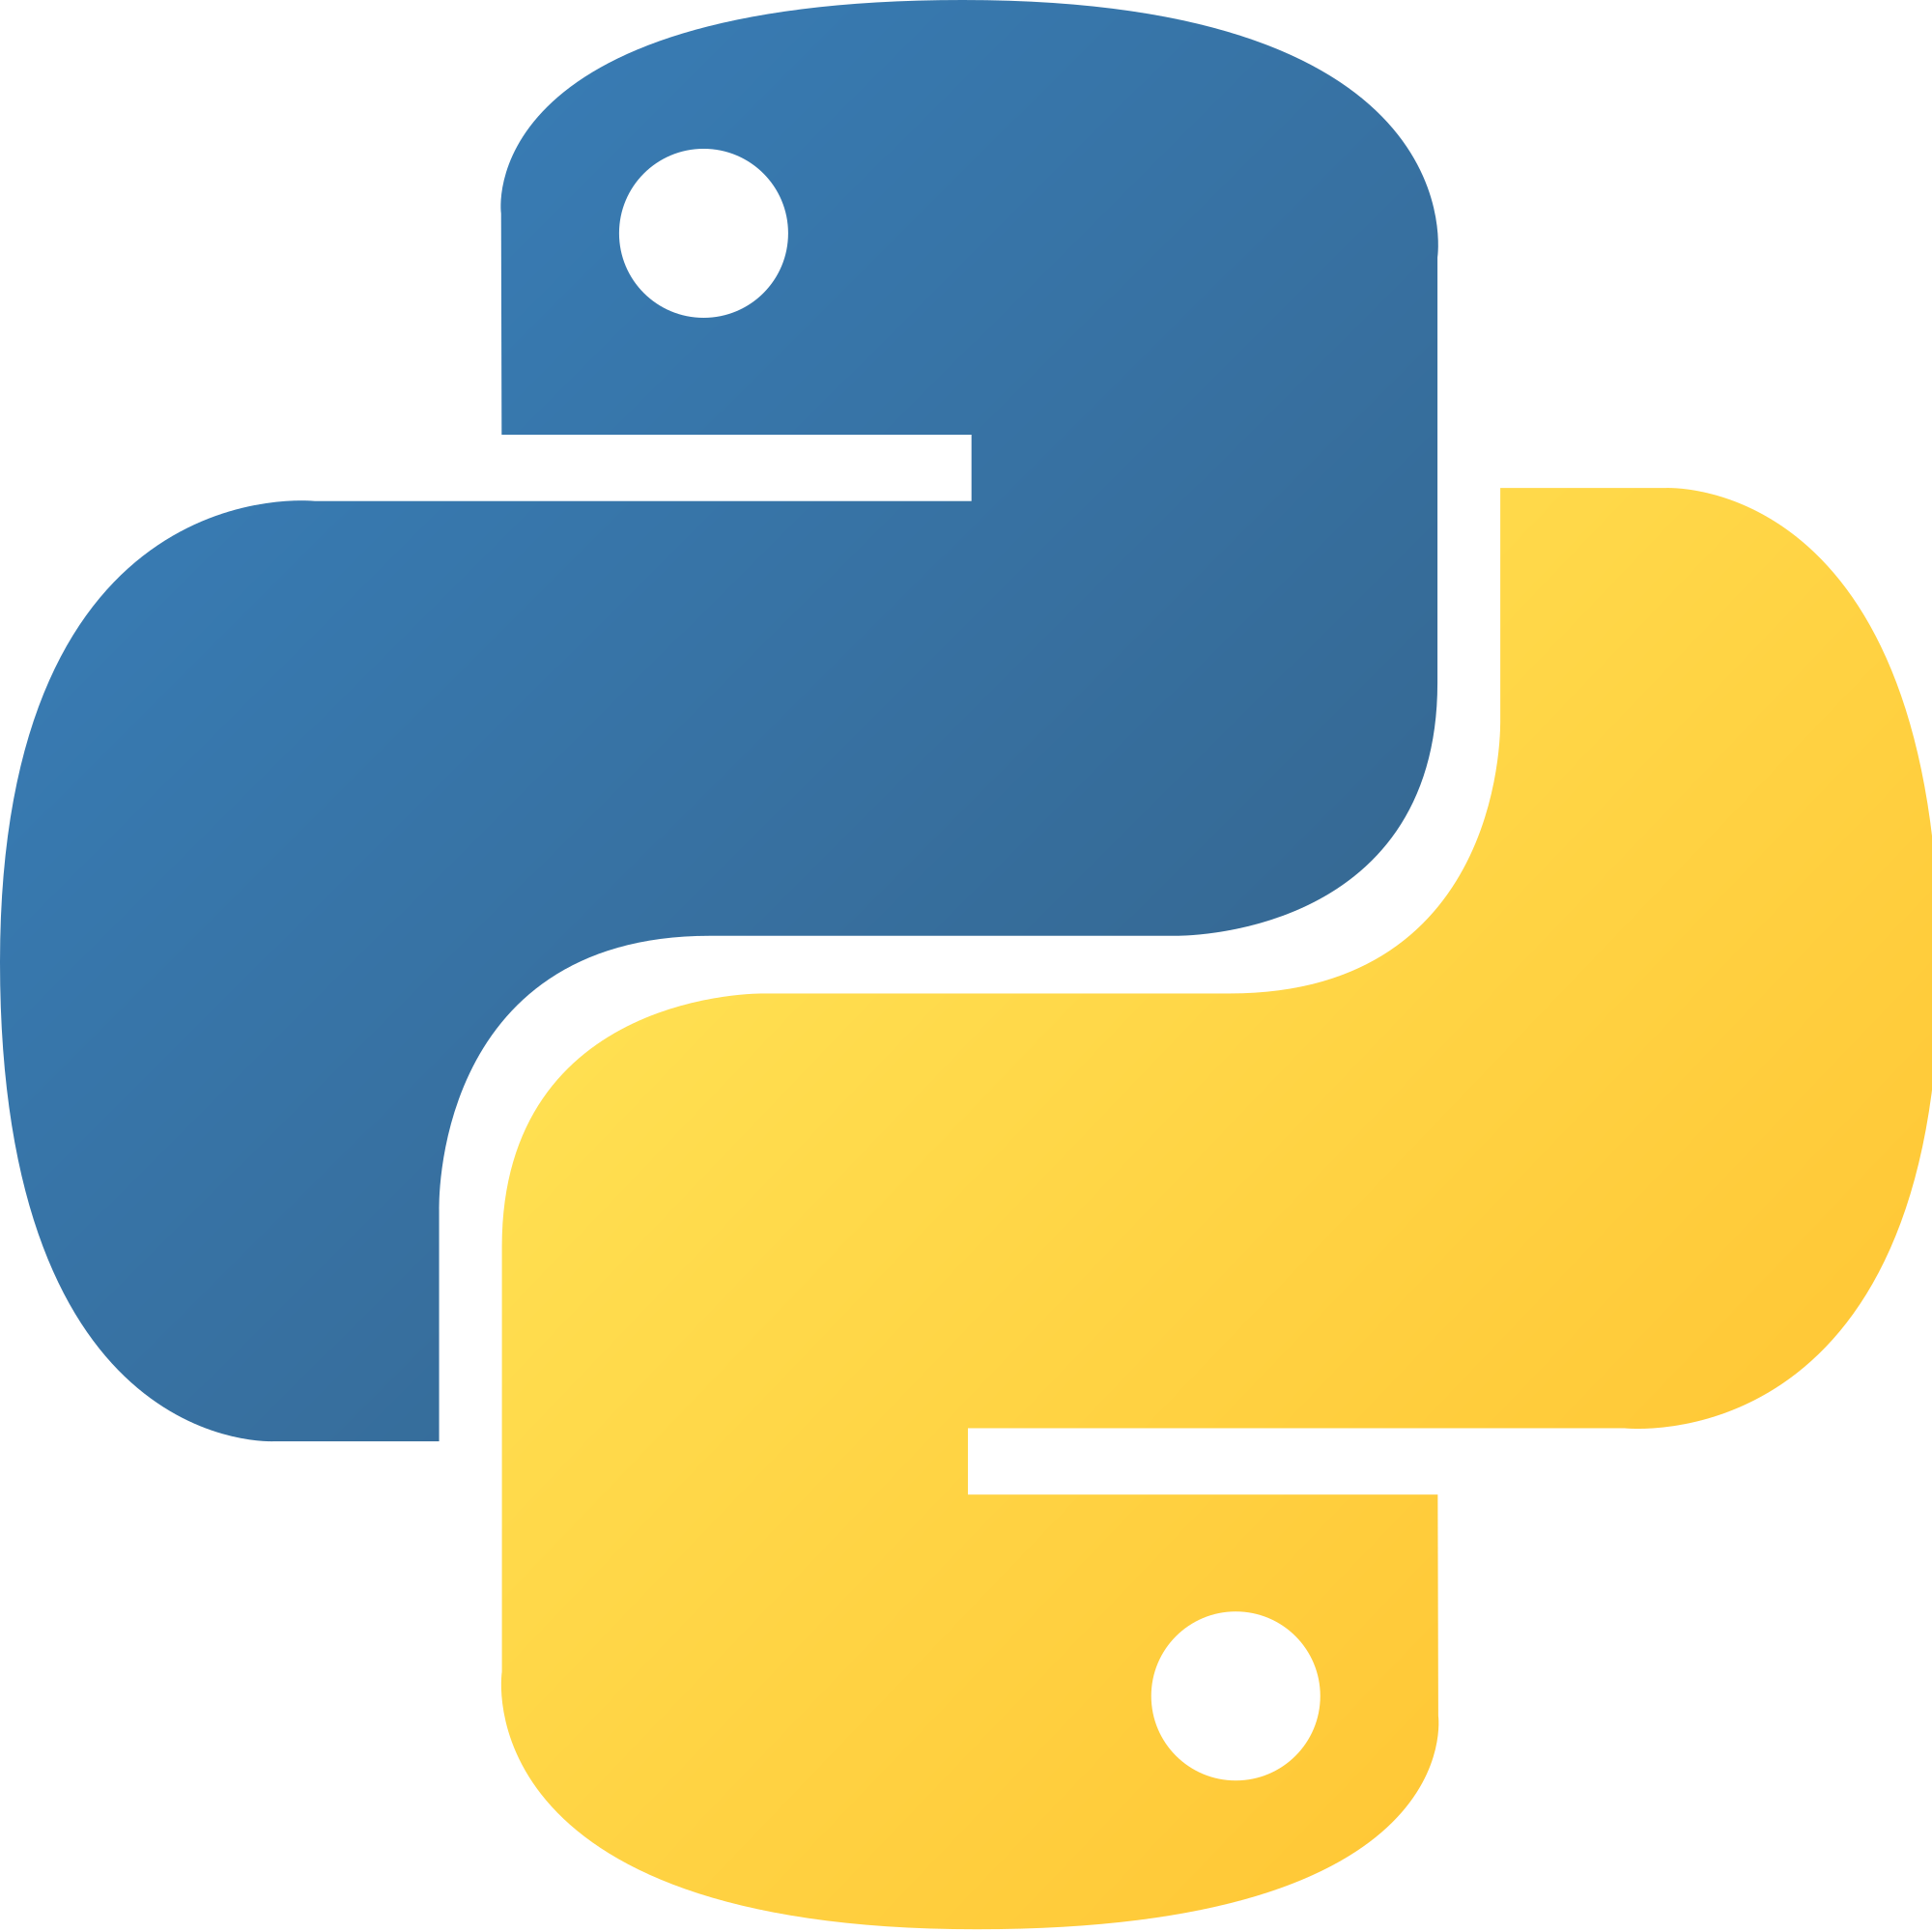
\includegraphics[scale=0.025]{PythonLogo.png} \\ \textbf{Python Programming}}}}
    \author{Nathan Stern}
    \pagenumbering{arabic}
    \usepackage{minted}
    \usepackage{color}   %May be necessary if you want to color links
    \usepackage{hyperref}
    \usepackage{indentfirst}
    \hypersetup{
        colorlinks=true, %set true if you want colored links
        linktoc=all,     %set to all if you want both sections and subsections linked
        linkcolor=black,  %choose some color if you want links to stand out
    }
\begin{document}
    \maketitle
    \tableofcontents
    \section{Introduction}
    
    This document is a quick introduction to programming in Python. This guide will cover everything that you will need to know in order to start programming in Python.

    \section{Hello, World!}

    This is the most basic program that any programmer will create when they first start learning a new language. It is usually the shortest program that they will ever make.
    
    \begin{minted}{Python}
    print ("Hello, World")
    \end{minted}

    In Python, the print function is very simple to use. You simpy have to type print() with the string that you want to print inside of the parenthesis with quotes around it.

    \section{Variables}

        Variables are a way of storing values in Python. There are many different kinds of variables that you can use in Python. The most common of these variable types are \textbf{Integers} and \textbf{Strings}. 

    \subsection{Integers}

    \subsection{Strings}

    \subsection{Arrays}
    
    \subsection{Dictionaries}

\end{document}